\documentclass[border=3pt]{standalone}
% Preâmbulo compartilhado pelos diagramas TikZ da aula 7 (Filtros Não Paramétricos)
\usepackage[T1]{fontenc}
\usepackage[utf8]{inputenc}
\usepackage{lmodern}
\usepackage{amsmath}
\usepackage{xcolor}
\usepackage{tikz}
\usetikzlibrary{arrows.meta,angles,quotes,decorations.pathmorphing,calc,
                positioning,shapes.geometric,shapes.misc,backgrounds,fit,
                math}

% Paleta (mesma dos SVGs originais)
\definecolor{dblue}{HTML}{2A5B8C}
\definecolor{dorange}{HTML}{B3541E}
\definecolor{dgreen}{HTML}{4A7C59}
\definecolor{dred}{HTML}{9C4B4B}
\definecolor{dcream}{HTML}{F4F1EA}
\definecolor{dshade}{HTML}{DDD7C9}

% Função gaussiana (não normalizada por padrão de escala visual)
\pgfmathdeclarefunction{gauss}{3}{%
  \pgfmathparse{1/(#3*sqrt(2*pi))*exp(-((#1-#2)^2)/(2*#3^2))}%
}

% Estilos comuns (prefixo d... para não colidir com chaves internas do pgf)
\tikzset{
  >={Stealth[length=2mm]},
  dguide/.style={gray!55, dashed, line width=0.4pt},
  daxis/.style={gray!60, line width=0.7pt, ->},
  dbody/.style={fill=black!3, draw=black!80, line width=1pt},
  dacc/.style={draw=dblue, line width=1pt},
  dlbl/.style={black!55, font=\small},
  dsub/.style={black!45, font=\footnotesize},
  dstate/.style={circle, draw=black!80, fill=dcream, line width=1pt,
                 minimum size=17mm, font=\large, inner sep=1pt},
  dobs/.style={circle, draw=black!80, fill=dshade, line width=1pt,
               minimum size=14mm, font=\large, inner sep=1pt},
  dbox/.style={rounded corners=2pt, draw=black!80, fill=dcream, line width=1pt,
               align=center, inner sep=6pt},
  dop/.style={circle, draw=black!80, fill=white, line width=1pt,
              minimum size=6mm, inner sep=0pt, font=\small},
  dtrans/.style={->, dblue, line width=1pt},
  dmeas/.style={->, dorange, line width=1pt},
  dcurve/.style={line width=1pt, dblue},
  dcurveb/.style={line width=1.4pt, dorange},
}

\begin{document}
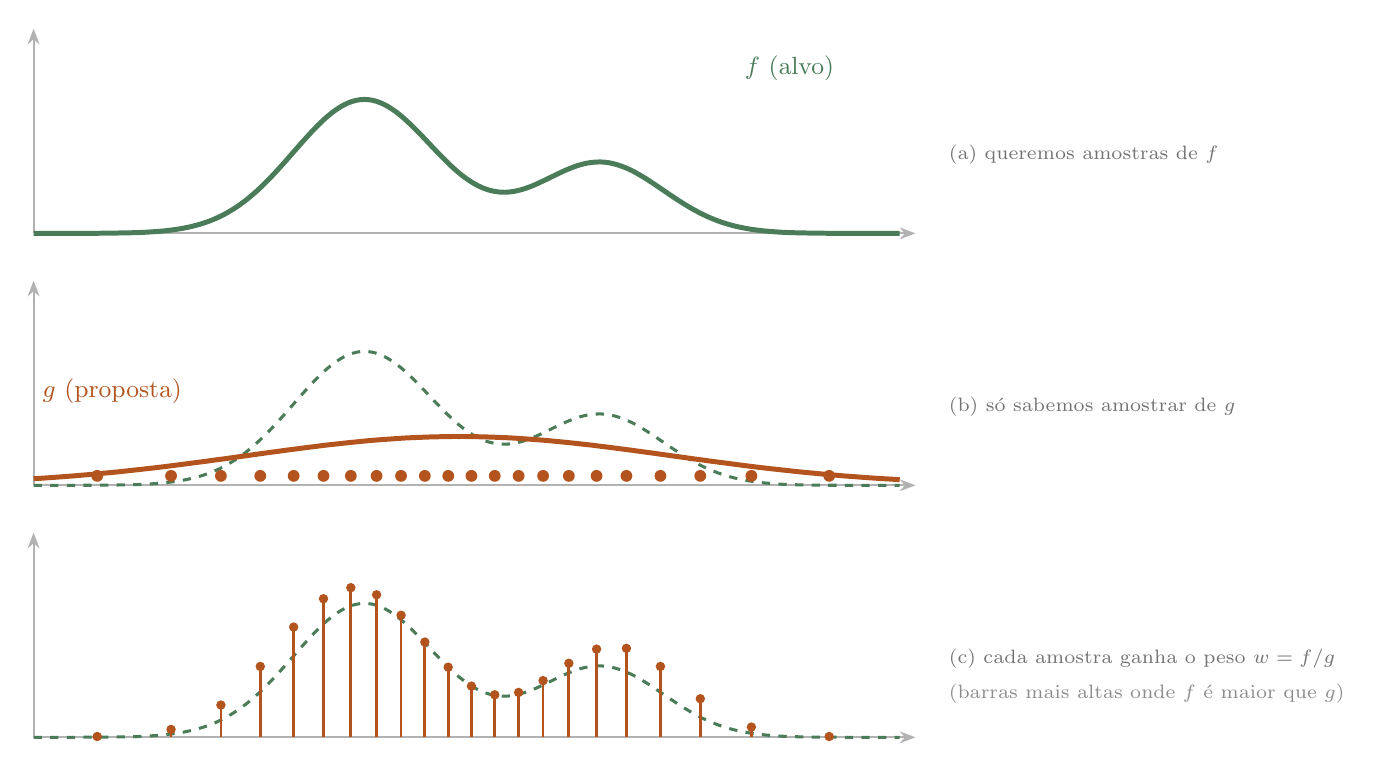
\begin{tikzpicture}[x=1cm,y=1cm]
\draw[daxis] (0,6.40) -- (11.2,6.40); \draw[daxis] (0,6.40) -- (0,9.00);
\draw[dgreen, line width=1.8pt] plot[smooth] coordinates {(0.000,6.400) (0.100,6.400) (0.200,6.400) (0.300,6.400) (0.400,6.400) (0.500,6.400) (0.600,6.401) (0.700,6.401) (0.800,6.401) (0.900,6.402) (1.000,6.403) (1.100,6.405) (1.200,6.407) (1.300,6.409) (1.400,6.413) (1.500,6.419) (1.600,6.426) (1.700,6.436) (1.800,6.449) (1.900,6.465) (2.000,6.486) (2.100,6.512) (2.200,6.544) (2.300,6.583) (2.400,6.630) (2.500,6.686) (2.600,6.750) (2.700,6.824) (2.800,6.907) (2.900,6.999) (3.000,7.099) (3.100,7.206) (3.200,7.317) (3.300,7.431) (3.400,7.545) (3.500,7.656) (3.600,7.761) (3.700,7.857) (3.800,7.940) (3.900,8.008) (4.000,8.059) (4.100,8.090) (4.200,8.101) (4.300,8.091) (4.400,8.061) (4.500,8.011) (4.600,7.945) (4.700,7.864) (4.800,7.771) (4.900,7.671) (5.000,7.566) (5.100,7.460) (5.200,7.357) (5.300,7.259) (5.400,7.170) (5.500,7.093) (5.600,7.029) (5.700,6.979) (5.800,6.945) (5.900,6.926) (6.000,6.922) (6.100,6.933) (6.200,6.956) (6.300,6.990) (6.400,7.032) (6.500,7.079) (6.600,7.128) (6.700,7.176) (6.800,7.220) (6.900,7.258) (7.000,7.286) (7.100,7.302) (7.200,7.307) (7.300,7.298) (7.400,7.275) (7.500,7.241) (7.600,7.196) (7.700,7.141) (7.800,7.080) (7.900,7.014) (8.000,6.946) (8.100,6.878) (8.200,6.812) (8.300,6.750) (8.400,6.692) (8.500,6.640) (8.600,6.595) (8.700,6.555) (8.800,6.522) (8.900,6.494) (9.000,6.472) (9.100,6.454) (9.200,6.440) (9.300,6.429) (9.400,6.421) (9.500,6.414) (9.600,6.410) (9.700,6.407) (9.800,6.405) (9.900,6.403) (10.000,6.402) (10.100,6.401) (10.200,6.401) (10.300,6.400) (10.400,6.400) (10.500,6.400) (10.600,6.400) (10.700,6.400) (10.800,6.400) (10.900,6.400) (11.000,6.400)};
\node[dgreen, font=\small] at (9.6,8.50) {$f$ (alvo)};
\node[dlbl, font=\scriptsize, anchor=west] at (11.5,7.40) {(a) queremos amostras de $f$};
\draw[daxis] (0,3.20) -- (11.2,3.20); \draw[daxis] (0,3.20) -- (0,5.80);
\draw[dgreen, line width=1.1pt, dashed] plot[smooth] coordinates {(0.000,3.200) (0.100,3.200) (0.200,3.200) (0.300,3.200) (0.400,3.200) (0.500,3.200) (0.600,3.201) (0.700,3.201) (0.800,3.201) (0.900,3.202) (1.000,3.203) (1.100,3.205) (1.200,3.207) (1.300,3.209) (1.400,3.213) (1.500,3.219) (1.600,3.226) (1.700,3.236) (1.800,3.249) (1.900,3.265) (2.000,3.286) (2.100,3.312) (2.200,3.344) (2.300,3.383) (2.400,3.430) (2.500,3.486) (2.600,3.550) (2.700,3.624) (2.800,3.707) (2.900,3.799) (3.000,3.899) (3.100,4.006) (3.200,4.117) (3.300,4.231) (3.400,4.345) (3.500,4.456) (3.600,4.561) (3.700,4.657) (3.800,4.740) (3.900,4.808) (4.000,4.859) (4.100,4.890) (4.200,4.901) (4.300,4.891) (4.400,4.861) (4.500,4.811) (4.600,4.745) (4.700,4.664) (4.800,4.571) (4.900,4.471) (5.000,4.366) (5.100,4.260) (5.200,4.157) (5.300,4.059) (5.400,3.970) (5.500,3.893) (5.600,3.829) (5.700,3.779) (5.800,3.745) (5.900,3.726) (6.000,3.722) (6.100,3.733) (6.200,3.756) (6.300,3.790) (6.400,3.832) (6.500,3.879) (6.600,3.928) (6.700,3.976) (6.800,4.020) (6.900,4.058) (7.000,4.086) (7.100,4.102) (7.200,4.107) (7.300,4.098) (7.400,4.075) (7.500,4.041) (7.600,3.996) (7.700,3.941) (7.800,3.880) (7.900,3.814) (8.000,3.746) (8.100,3.678) (8.200,3.612) (8.300,3.550) (8.400,3.492) (8.500,3.440) (8.600,3.395) (8.700,3.355) (8.800,3.322) (8.900,3.294) (9.000,3.272) (9.100,3.254) (9.200,3.240) (9.300,3.229) (9.400,3.221) (9.500,3.214) (9.600,3.210) (9.700,3.207) (9.800,3.205) (9.900,3.203) (10.000,3.202) (10.100,3.201) (10.200,3.201) (10.300,3.200) (10.400,3.200) (10.500,3.200) (10.600,3.200) (10.700,3.200) (10.800,3.200) (10.900,3.200) (11.000,3.200)};
\draw[dorange, line width=1.8pt] plot[smooth] coordinates {(0.000,3.284) (0.100,3.290) (0.200,3.297) (0.300,3.304) (0.400,3.312) (0.500,3.319) (0.600,3.328) (0.700,3.336) (0.800,3.345) (0.900,3.355) (1.000,3.364) (1.100,3.374) (1.200,3.385) (1.300,3.396) (1.400,3.407) (1.500,3.418) (1.600,3.430) (1.700,3.442) (1.800,3.455) (1.900,3.468) (2.000,3.481) (2.100,3.494) (2.200,3.507) (2.300,3.521) (2.400,3.534) (2.500,3.548) (2.600,3.562) (2.700,3.576) (2.800,3.590) (2.900,3.604) (3.000,3.618) (3.100,3.631) (3.200,3.645) (3.300,3.658) (3.400,3.671) (3.500,3.684) (3.600,3.696) (3.700,3.709) (3.800,3.720) (3.900,3.731) (4.000,3.742) (4.100,3.752) (4.200,3.762) (4.300,3.771) (4.400,3.779) (4.500,3.786) (4.600,3.793) (4.700,3.800) (4.800,3.805) (4.900,3.809) (5.000,3.813) (5.100,3.816) (5.200,3.818) (5.300,3.820) (5.400,3.820) (5.500,3.820) (5.600,3.818) (5.700,3.816) (5.800,3.813) (5.900,3.809) (6.000,3.805) (6.100,3.800) (6.200,3.793) (6.300,3.786) (6.400,3.779) (6.500,3.771) (6.600,3.762) (6.700,3.752) (6.800,3.742) (6.900,3.731) (7.000,3.720) (7.100,3.709) (7.200,3.696) (7.300,3.684) (7.400,3.671) (7.500,3.658) (7.600,3.645) (7.700,3.631) (7.800,3.618) (7.900,3.604) (8.000,3.590) (8.100,3.576) (8.200,3.562) (8.300,3.548) (8.400,3.534) (8.500,3.521) (8.600,3.507) (8.700,3.494) (8.800,3.481) (8.900,3.468) (9.000,3.455) (9.100,3.442) (9.200,3.430) (9.300,3.418) (9.400,3.407) (9.500,3.396) (9.600,3.385) (9.700,3.374) (9.800,3.364) (9.900,3.355) (10.000,3.345) (10.100,3.336) (10.200,3.328) (10.300,3.319) (10.400,3.312) (10.500,3.304) (10.600,3.297) (10.700,3.290) (10.800,3.284) (10.900,3.278) (11.000,3.272)};
\node[dorange, font=\small] at (1.0,4.40) {$g$ (proposta)};
\fill[dorange] (0.808,3.32) circle (0.075);
\fill[dorange] (1.746,3.32) circle (0.075);
\fill[dorange] (2.379,3.32) circle (0.075);
\fill[dorange] (2.879,3.32) circle (0.075);
\fill[dorange] (3.303,3.32) circle (0.075);
\fill[dorange] (3.682,3.32) circle (0.075);
\fill[dorange] (4.029,3.32) circle (0.075);
\fill[dorange] (4.356,3.32) circle (0.075);
\fill[dorange] (4.667,3.32) circle (0.075);
\fill[dorange] (4.969,3.32) circle (0.075);
\fill[dorange] (5.266,3.32) circle (0.075);
\fill[dorange] (5.561,3.32) circle (0.075);
\fill[dorange] (5.857,3.32) circle (0.075);
\fill[dorange] (6.160,3.32) circle (0.075);
\fill[dorange] (6.471,3.32) circle (0.075);
\fill[dorange] (6.798,3.32) circle (0.075);
\fill[dorange] (7.150,3.32) circle (0.075);
\fill[dorange] (7.529,3.32) circle (0.075);
\fill[dorange] (7.961,3.32) circle (0.075);
\fill[dorange] (8.467,3.32) circle (0.075);
\fill[dorange] (9.116,3.32) circle (0.075);
\fill[dorange] (10.104,3.32) circle (0.075);
\node[dlbl, font=\scriptsize, anchor=west] at (11.5,4.20) {(b) só sabemos amostrar de $g$};
\draw[daxis] (0,0.00) -- (11.2,0.00); \draw[daxis] (0,0.00) -- (0,2.60);
\draw[dgreen, line width=1.1pt, dashed] plot[smooth] coordinates {(0.000,0.000) (0.100,0.000) (0.200,0.000) (0.300,0.000) (0.400,0.000) (0.500,0.000) (0.600,0.001) (0.700,0.001) (0.800,0.001) (0.900,0.002) (1.000,0.003) (1.100,0.005) (1.200,0.007) (1.300,0.009) (1.400,0.013) (1.500,0.019) (1.600,0.026) (1.700,0.036) (1.800,0.049) (1.900,0.065) (2.000,0.086) (2.100,0.112) (2.200,0.144) (2.300,0.183) (2.400,0.230) (2.500,0.286) (2.600,0.350) (2.700,0.424) (2.800,0.507) (2.900,0.599) (3.000,0.699) (3.100,0.806) (3.200,0.917) (3.300,1.031) (3.400,1.145) (3.500,1.256) (3.600,1.361) (3.700,1.457) (3.800,1.540) (3.900,1.608) (4.000,1.659) (4.100,1.690) (4.200,1.701) (4.300,1.691) (4.400,1.661) (4.500,1.611) (4.600,1.545) (4.700,1.464) (4.800,1.371) (4.900,1.271) (5.000,1.166) (5.100,1.060) (5.200,0.957) (5.300,0.859) (5.400,0.770) (5.500,0.693) (5.600,0.629) (5.700,0.579) (5.800,0.545) (5.900,0.526) (6.000,0.522) (6.100,0.533) (6.200,0.556) (6.300,0.590) (6.400,0.632) (6.500,0.679) (6.600,0.728) (6.700,0.776) (6.800,0.820) (6.900,0.858) (7.000,0.886) (7.100,0.902) (7.200,0.907) (7.300,0.898) (7.400,0.875) (7.500,0.841) (7.600,0.796) (7.700,0.741) (7.800,0.680) (7.900,0.614) (8.000,0.546) (8.100,0.478) (8.200,0.412) (8.300,0.350) (8.400,0.292) (8.500,0.240) (8.600,0.195) (8.700,0.155) (8.800,0.122) (8.900,0.094) (9.000,0.072) (9.100,0.054) (9.200,0.040) (9.300,0.029) (9.400,0.021) (9.500,0.014) (9.600,0.010) (9.700,0.007) (9.800,0.005) (9.900,0.003) (10.000,0.002) (10.100,0.001) (10.200,0.001) (10.300,0.000) (10.400,0.000) (10.500,0.000) (10.600,0.000) (10.700,0.000) (10.800,0.000) (10.900,0.000) (11.000,0.000)};
\draw[dorange, line width=1pt] (0.808,0.00) -- (0.808,0.01); \fill[dorange] (0.808,0.01) circle (0.06);
\draw[dorange, line width=1pt] (1.746,0.00) -- (1.746,0.10); \fill[dorange] (1.746,0.10) circle (0.06);
\draw[dorange, line width=1pt] (2.379,0.00) -- (2.379,0.41); \fill[dorange] (2.379,0.41) circle (0.06);
\draw[dorange, line width=1pt] (2.879,0.00) -- (2.879,0.90); \fill[dorange] (2.879,0.90) circle (0.06);
\draw[dorange, line width=1pt] (3.303,0.00) -- (3.303,1.40); \fill[dorange] (3.303,1.40) circle (0.06);
\draw[dorange, line width=1pt] (3.682,0.00) -- (3.682,1.76); \fill[dorange] (3.682,1.76) circle (0.06);
\draw[dorange, line width=1pt] (4.029,0.00) -- (4.029,1.90); \fill[dorange] (4.029,1.90) circle (0.06);
\draw[dorange, line width=1pt] (4.356,0.00) -- (4.356,1.81); \fill[dorange] (4.356,1.81) circle (0.06);
\draw[dorange, line width=1pt] (4.667,0.00) -- (4.667,1.55); \fill[dorange] (4.667,1.55) circle (0.06);
\draw[dorange, line width=1pt] (4.969,0.00) -- (4.969,1.21); \fill[dorange] (4.969,1.21) circle (0.06);
\draw[dorange, line width=1pt] (5.266,0.00) -- (5.266,0.89); \fill[dorange] (5.266,0.89) circle (0.06);
\draw[dorange, line width=1pt] (5.561,0.00) -- (5.561,0.65); \fill[dorange] (5.561,0.65) circle (0.06);
\draw[dorange, line width=1pt] (5.857,0.00) -- (5.857,0.54); \fill[dorange] (5.857,0.54) circle (0.06);
\draw[dorange, line width=1pt] (6.160,0.00) -- (6.160,0.57); \fill[dorange] (6.160,0.57) circle (0.06);
\draw[dorange, line width=1pt] (6.471,0.00) -- (6.471,0.72); \fill[dorange] (6.471,0.72) circle (0.06);
\draw[dorange, line width=1pt] (6.798,0.00) -- (6.798,0.94); \fill[dorange] (6.798,0.94) circle (0.06);
\draw[dorange, line width=1pt] (7.150,0.00) -- (7.150,1.12); \fill[dorange] (7.150,1.12) circle (0.06);
\draw[dorange, line width=1pt] (7.529,0.00) -- (7.529,1.13); \fill[dorange] (7.529,1.13) circle (0.06);
\draw[dorange, line width=1pt] (7.961,0.00) -- (7.961,0.90); \fill[dorange] (7.961,0.90) circle (0.06);
\draw[dorange, line width=1pt] (8.467,0.00) -- (8.467,0.49); \fill[dorange] (8.467,0.49) circle (0.06);
\draw[dorange, line width=1pt] (9.116,0.00) -- (9.116,0.13); \fill[dorange] (9.116,0.13) circle (0.06);
\draw[dorange, line width=1pt] (10.104,0.00) -- (10.104,0.01); \fill[dorange] (10.104,0.01) circle (0.06);
\node[dlbl, font=\scriptsize, anchor=west] at (11.5,1.00) {(c) cada amostra ganha o peso $w=f/g$};
\node[dsub, font=\scriptsize, anchor=west] at (11.5,0.55) {(barras mais altas onde $f$ é maior que $g$)};
\end{tikzpicture}
\end{document}
